\section{Cultivos hidropónicos}
Históricamente, la agricultura tradicional ha utilizado el suelo como medio principal para el crecimiento de plantas gracias a su alta concentración de minerales y nutrientes esenciales para el desarrollo de hojas y frutos. Debido al crecimiento poblacional observado en los últimos siglos, las metodologías de agricultura tradicional han extraído una cantidad considerable de nutrientes del suelo, reduciendo su productividad y aumentando su dependencia de fertilizantes añadidos. 

A mediados del siglo pasado, se empezaron a investigar una técnicas de agricultura con tal de eliminar la dependencia del suelo para el crecimiento de las plantas. Una de las soluciones encontradas fueron los cultivos hidropónicos los cuales no dependen de un sustrato para entregar minerales y nutrientes esenciales para el crecimiento de las plantas, sino se aprovechan de una solución de estos en agua para maximizar la absorción por medio de las raíces \cite{raviv_soilless_2019}. Los sistemas hidropónicos se caracterizan por su bajo consumo de agua, alta eficiencia de espacio y altos niveles de productividad. Se destaca que estos sistemas no dependen de las condiciones climáticas de la región, al encontrarse en un entorno controlado, como un invernadero. Esto permite una producción constante a lo largo del año la cual no es susceptible a sequías o inundaciones. Adicionalmente, al no depender del suelo, estos sistemas se pueden expandir de manera vertical, lo cual aumenta la producción de plantas por metro cuadrado utilizado. Estas características han vuelto a la hidroponía una de las soluciones más prometedoras en el contexto del crecimiento urbano y poblacional visto en el siglo XXI. Otra de las grandes ventajas de contar con un entorno cerrado y controlable, es que los cultivos hidropónicos raras veces se encuentran expuestos a pestes o enfermedades relacionadas al suelo. Sin embargo, su dependencia de un control constante y riguroso de parámetros, hace de esta metodología de cultivo susceptible a pérdidas por mal manejo del sistema \cite{raviv_soilless_2019}.

\section{Solución nutritiva re-circulante (NFT)}
La hidroponía cuenta con una gran variedad de métodos ideados con la finalidad de maximizar espacio, eficiencia de distribución de materiales y otros parámetros de crecimiento de las plantas \cite{rajaseger_hydroponics_2023}. La principal diferencia entre los métodos de cultivo hidropónico consiste en los métodos de irrigación. El método de solución nutritiva re-circulante (\textit{Nutrient Film Technique}), también conocido como método NFT, utiliza un sistema de irrigación que genera una película delgada de agua con nutrientes que fluye sobre las raíces de las plantas. Tradicionalmente, estos sistemas se implementan con una serie de canaletas o tuberías colocadas a una inclinación de entre 0.3\% y 2\% \cite{van_os_technical_2019}. Una de las características más retadoras del método NFT consiste en el control de parámetros, como lo son los niveles de pH de la solución, su temperatura, oxígeno disuelto y saturación de nutrientes \cite{baiyin_flow_rate_2021}. Adicionalmente, varios estudios han demostrado que la tasa de flujo de la solución en el sistema se encuentra fuertemente relacionada con el rendimiento del crecimiento de las plantas. En el caso de las lechugas, Al-Tawaha y colaboradores encontraron que un flujo de 20 L/minuto fue óptimo para el desarrollo de las plantas, llevando a un mayor rendimiento \cite{al-tawaha_flow_rate_nft_2018}. Finalmente, es importante destacar que este sistema requiere que las plantas sean germinadas en un espacio separado, antes de que puedan ser introducidas al sistema.

\begin{figure}[H]
	\centering
	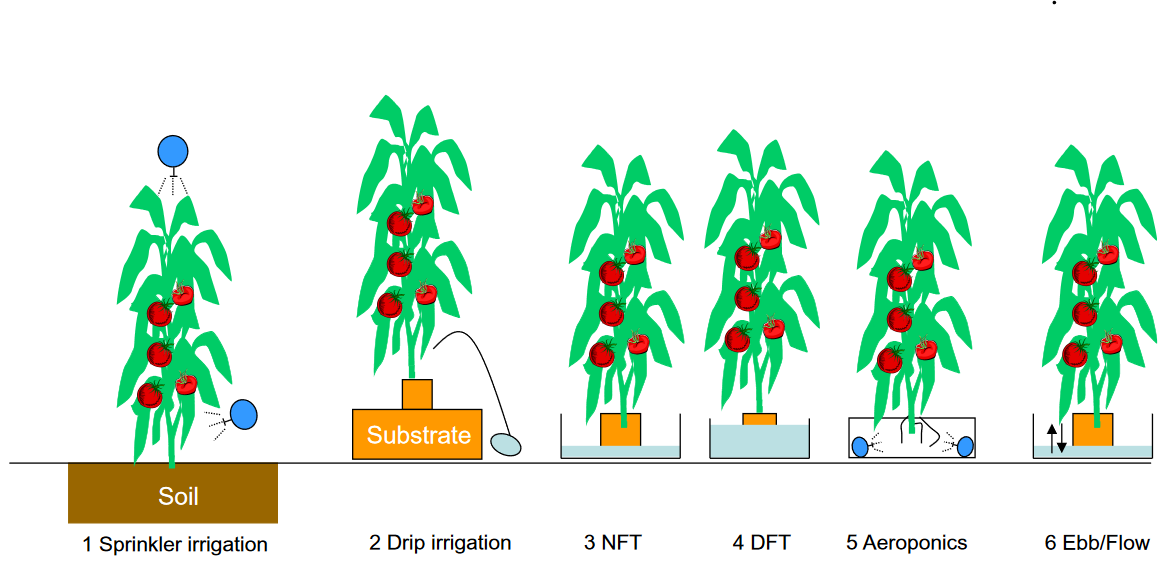
\includegraphics[scale= 0.35]{Figura_5_metodos_irrigacion.png}
	\caption{Variedad de métodos de irrigación para cultivos \cite{van_os_technical_2019}.}
	\label{fig:mesh5}
\end{figure}

\begin{figure}[H]
	\centering
	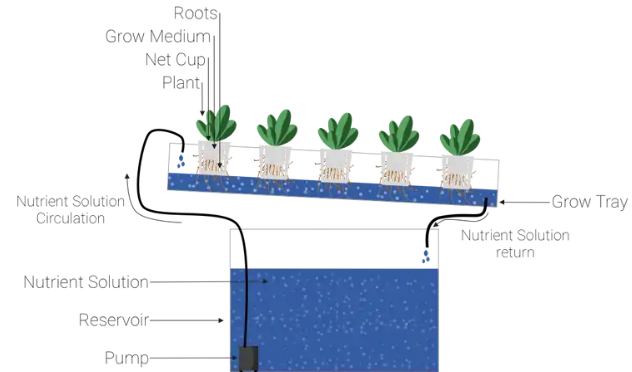
\includegraphics[scale= 0.45]{Figura_6_sistema_nft.png}
	\caption{Diagrama simplificado de metodología NFT para cultivos hidropónicos \cite{NutrientFilmTechnique_2023}.}
	\label{fig:mesh6}
\end{figure}

\section{Solución de nutrientes}
Acceso constante a luz solar, agua, oxígeno y dióxido de carbono es esencial para la supervivencia de las plantas. Sin embargo, esto no es lo único que requieren para su crecimiento. Normalmente, las plantas obtienen la mayoría de los minerales y nutrientes necesarios para su crecimiento del suelo, el cual, a lo largo de varios años por procesos naturales, ha acumulado en diferentes cantidades. Las plantas requieren de 13 nutrientes minerales necesarios para su desarrollo y crecimiento adecuado. Sus características de crecimiento y la calidad de las plantas estarán definidas por el porcentaje de nutrientes que tengan disponibles y que sean capaces de absorber \cite{marulanda_huerta_2003}. Estos nutrientes se pueden dividir en tres categorías según la función que cumple cada elemento. La primera categoría se conoce como los macro-nutrientes, estos son nutrientes que las plantas requieren en altas cantidades pues son esenciales para el desarrollo de las estructuras fundamentales para su crecimiento. En este grupo se encuentran el Nitrato requerido para el desarrollo de hojas y tallos; el Fósforo, requerido para el desarrollo de raíces, la formación de semillas y la maduración de frutos; y el Potasio, requerido para el desarrollo de frutos y la acumulación de nutrientes en la planta \cite{marulanda_huerta_2003}.

La segunda categoría consiste en minerales requeridos para el correcto desarrollo de la planta, sin embargo, estos son requeridos en cantidades más bajas por lo que se conocen como elementos secundarios. Entre estos se encuentra el Calcio, el cual activa la formación de raíces, especialmente en las primeras etapas de desarrollo y neutraliza las sustancias tóxicas producidas por la planta. También se encuentra el Azufre, el cual es esencial en la producción de proteínas, mejora el crecimiento de la planta y facilita el desarrollo de semillas. Adicionalmente, en este grupo se cuenta con el Magnesio, el cual es fundamental para las plantas porque es requerido para la creación de clorofila y las azúcares que requieren para vivir, adicionalmente es utilizado para regular los nutrientes dentro de la planta y fomenta la creación de aceites y grasas \cite{marulanda_huerta_2003}. Finalmente, se cuenta con una serie de micro-nutrientes, los cuales cumplen una gran variedad de funciones que facilitan el desarrollo de la planta y aseguran un mayor rendimiento de la misma. Estos se detallan a continuación \cite{atlas_scientific_nutrient_2023}:

\begin{itemize}
	\item Cloro\\
	Utilizado para facilitar el proceso de fotosíntesis y regular los niveles de sales y líquido en las células lo cual asegura una planta fresca y saludable.
	\item Molibdeno\\
	Elemento esencial para la fijación de nitrógeno y utilizado en el proceso de conversión de nitrato a amoniaco.
	\item Manganeso\\
	De gran utilidad para aumentar la resiliencia de las plantas ante situaciones de alto estrés, y utilizado en el proceso de activación de enzimas.
	\item Zinc\\
	Requerido para la síntesis de hormonas de crecimiento y el desarrollo de raíces.
	\item Boro\\
	Apoya en el proceso de crecimiento al fomentar la división de células y el metabolismo de carbohidrátos.
	\item Hierro\\
	Esencial para la transferencia de energía entre células y la producción de clorofila.
	\item Cobre\\
	Mejora la estructura de las plantas al reforzar las paredes celulares mediante la formación de lignina. Esencial en la creación de estructuras maderosas.
\end{itemize}

El correcto suministro y balance de estos componentes en un sistema hidropónico es esencial para asegurar el crecimiento adecuado y el rendimiento de los cultivos. Ahora bien, su aplicación y control de manera individual sería sumamente difícil, por esta razón, se han desarrollado fórmulas para proveer estos nutrientes en un sistema hidropónico. En la industria estas soluciones se conocen como solución concentrada A y B, donde la primera cuenta con los macro-nutrientes y nutrientes secundarios, mientras que la segunda cuenta con los micro-nutrientes \cite{marulanda_huerta_2003}. Estas soluciones pueden ser creadas de manera independiente, o se pueden adquirir en el mercado. Es importante destacar que los porcentajes de concentración a utilizar en el sistema hidropónico dependerá del tipo de cultivo y sus requisitos. Por ejemplo, un cultivo de hortalizas requerirá mayores porcentajes de nitrógeno y nutrientes secundarios, mientras que plantas con flores y frutos, requerirán una mayor concentración de fósforo y potasio. Así mismo, cambios en la temperatura requerirán de un ajuste en la concentración total en el agua, puesto que, a mayores temperaturas, las plantas aumentarán su consumo de agua, mas no su dependencia en minerales, mientras que a menores temperaturas, se ve lo opuesto \cite{marulanda_huerta_2003}.

\section{Características de la solución nutritiva del cilantro}
El cilantro es una hierba bastante versátil la cual requiere de una baja cantidad de nutrientes con tal de presentar una productividad significativa. De los nutrientes mencionados anteriormente, el cilantro requiere únicamente un control rigoroso de los macro-nutrientes principales así como una baja cantidad de Calcio y Magnesio \cite{letpot_nodate}. Este control de macro-nutrientes va de la mano con una regulación cuidadosa de la temperatura del agua. Esto pues, en diferentes rangos de temperatura varía la necesidad de nutrientes así como su facilidad de absorción \cite{voogt_nutrient_2019}.

Según el estudio realizado por Currey y colaboradores, uno de los factores que más interfiere en el crecimiento y desarrollo del cilantro es la cantidad de fotones que reciben las plantas durante el día. Esto se puede traducir a la cantidad de horas de luz que requieren para su crecimiento óptimo, el cual se encuentra en un rango de 12 a 16 horas de luz diarias \cite{letpot_nodate}. Una conclusión importante del estudio de Currey y colaboradores es que si bien la concentración de luz disponible para la planta aumenta su productividad, no es necesario realizar un ajuste de la densidad de nutrientes debido al aumento en concentración de luz \cite{currey_nutrient_2019}. A continuación se detallan los parámetros del agua requeridos para el correcto desarrollo del cilantro en un sistema hidropónico:

\begin{table}[H]
	\centering
	\begin{tabular}{|c|c|}
		\hline
		\multicolumn{2}{|c|}{\textbf{Características de la solución nutritiva}}\\ \hline
		Concentración de nutrientes: & 1.2 a 1.8 mS/cm \\ \hline
		Potencia de hidrógeno (pH): & 5.5 a 6.7 \\ \hline
		Temperatura del agua: & 15 a 20 °C \\ \hline
		Nutrientes requeridos: & Nitrógeno, fósforo, potasio, calcio y magnesio \\ \hline
		Concentración de nutrientes: & NPK 15:15:15\\ \hline
		Nutrientes adicionales: &  0.5\% Nitrato de calcio y 0.5\% Sulfato de magnesio\\ \hline
		Tiempo de crecimiento: & 50 a 55 días\\ \hline
		Espacio entre plantas: & 18 cm \\ \hline
	\end{tabular}
	\caption{Parámetros esenciales para el crecimiento de Cilantro en sistemas hidropónicos \cite{mondol_use_2023} \cite{letpot_nodate}.}
	\label{Cuadro0}
\end{table}

\section{Monitoreo de parámetros para el crecimiento de plantas}
Como se detalló anteriormente, los cultivos hidropónicos requieren de un control constante y preciso de una gran variedad de parámetros. El monitoreo adecuado de parámetros como el nivel de oxigenación del agua, la cantidad de nutrientes, el nivel de acidez de la solución, la temperatura del ambiente, temperatura del agua, y el nivel de humedad son esenciales para asegurar el crecimiento óptimo de las plantas. Tradicionalmente, estos parámetros se miden con una serie de pruebas químicas o sensores independientes. A continuación, se detallan los diferentes sensores que se pueden utilizar en un cultivo hidropónico para medir los parámetros del agua así como la importancia de cada uno de dichos parámetros.

\subsection{Oxígeno disuelto en agua}
Los sistemas hidropónicos se enfrentan a varios retos, entre estos, la cantidad de oxígeno disuelto en la solución de nutrientes. Este parámetro es esencial para el desarrollo saludable de las raíces, puesto que con bajos niveles de oxígeno, estas pueden experimentar una enfermedad conocida como hipoxia. Según el estudio realizado por Roosta, los niveles de oxígeno están directamente relacionados no sólo con el crecimiento de las raíces, sino también con los procesos fotosintéticos y de crecimiento de los cultivos hidropónicos. Este parámetro afecta la absorción de Nitrógeno ya sea que se encuentre en la forma de sales de nitratos o amoníacos\cite{roosta_responses_2024}. La concentración de oxígeno disuelto se mide en mg/L, lo cual se puede lograr con una gran variedad de sensores.

\subsection{\textit{SEN0237 Gravity Analog Dissolved Oxygen Sensor} de \textit{DFRobot}}
El sensor analógico de oxígeno disuelto consiste en una sonda galvánica equipada con un electrodo el cual junto con una solución de hidróxido de sodio, también conocido como sosa cáustica, es capaz de detectar la concentración de oxígeno disuelto en agua. Dicho sensor debe ser calibrado antes de que se pueda utilizar, sin embargo, dicho proceso es relativamente sencillo \cite{DFRobot_DOsensor}. 

Según el fabricante, el sensor se puede calibrar utilizando un método de punto singular o de doble punto. El primer proceso requiere de la preparación de una solución de oxígeno concentrado en agua, esto se puede lograr utilizando un batidor o con una bomba de aire inmersa en el agua destilada durante 10 minutos. Una vez terminen los 10 minutos, se espera a que dejen de salir burbujas, y se sumerge la sonda en la solución. Se mantienen mezclando la solución lentamente para evitar burbujas hasta que el nivel de voltaje se estabilice y se guardan los valores de temperatura y voltaje como punto de saturación. El proceso de doble punto es similar al descrito anteriormente, sin embargo, requiere de dos soluciones a dos temperaturas diferentes. Se recomienda que una se encuentre alrededor de 5°C y la otra entre los 35° y 38°C \cite{DFRobot_DOsensor}. 

A continuación, se detallan las características del sensor:

\begin{table}[H]
	\centering
	\begin{tabular}{|c|c|}
		\hline
		\multicolumn{2}{|c|}{\textbf{Sonda del sensor de oxígeno disuelto}}\\ \hline
		Rango de detección: & 0 a 20 mg/L \\ \hline
		Rango de temperatura: & 0 a 40 °C \\ \hline
		Tiempo de respuesta: & 90 segundos a 25 °C \\ \hline
		Rango de presión: & 0 a 50 PSI \\ \hline
		Vida útil del electrodo: & 1 año (bajo condiciones normales de uso) \\ \hline
		Tiempo de reemplazo de membrana: & Cada 4 a 5 meses en agua clara \\ \hline
		Tiempo de reemplazo de solución: & Una vez al mes \\ \hline
		Largo del cable: & 2 metros \\ \hline
		Tipo de conector de la sonda: & BNC \\ \hline
		\multicolumn{2}{|c|}{\textbf{Placa de conversión de señales del sensor}}\\ \hline 
		Voltaje de alimentación: & 3.3 a 5.5 VDC \\ \hline
		Voltaje de señal de salida: & 0 a 3.3 VDC \\ \hline
		Cable de conexión: & BNC \\ \hline
		Conector de señal: & Interfaz PH2.0 - 3 pin \\ \hline
		Dimensiones: & 42mm $\times$ 32mm (1.65in $\times$ 1.26in) \\ \hline
	\end{tabular}
	\caption{Características de funcionamiento del sensor SEN0237 de \textit{DFRobot}.}
	\label{Cuadro1}
\end{table}

\begin{figure}[H]
	\centering
	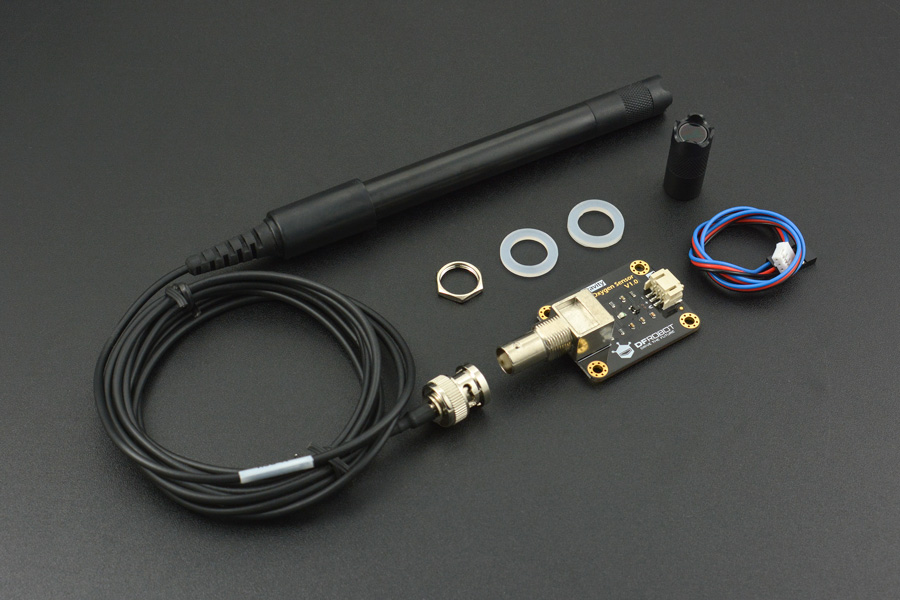
\includegraphics[scale= 0.25]{Figura_7_sensor_oxigeno.jpg}
	\caption{Sensor analógico de oxígeno disuelto \cite{DFRobot_DOsensor}.}
	\label{fig:mesh7}
\end{figure}


\subsection{Sensor de electro conductividad (EC)}
Las soluciones de nutrientes requeridas para el crecimiento de las plantas cuentan con compuestos en la forma de sales, las cuales afectan la conductividad eléctrica del agua. Estas variaciones permiten utilizar los sensores de electro conductividad para determinar de manera aproximada la concentración de solución nutritiva en el agua de riego. La conductividad, medida en mS/cm (mili sievers por centímetro), es una propiedad de los materiales la cual se define como el inverso de la resistencia. El sensor \textit{DFR0300 Gravity Analog Electrical Conductividy Sensor} de \textit{DFRobot} cuenta con dos electrodos los cuales son introducidos en el agua para determinar su conductividad eléctrica, esta señal es luego convertida a un valor de voltaje analógico y transmitido a un microcontrolador \cite{DFRobot_ECsensor}. A continuación se detallan las características del sensor:

\begin{table}[H]
	\centering
	\begin{tabular}{|c|c|}
		\hline
		\multicolumn{2}{|c|}{\textbf{Sonda del sensor de conductividad eléctrica}}\\ \hline
		Constante de celda: & 1.0 \\ \hline
		Rango de detección admisible: & 0 a 20 mS/cm \\ \hline
		Rango de detección recomendado: & 1 a 15 mS/cm \\ \hline
		Rango de temperatura: & 0 a 40 °C \\ \hline
		Vida útil del sensor: & Más de 6 meses según frecuencia de uso \\ \hline
		Largo del cable: & 100 cm \\ \hline
		\multicolumn{2}{|c|}{\textbf{Placa de conversión de señales del sensor}}\\ \hline 
		Voltaje de alimentación: & 3.0 a 5.0 VDC \\ \hline
		Voltaje de señal de salida: & 0 a 3.4 VDC \\ \hline
		Certeza de medición: & $\pm 5\%$ F.S. \\ \hline
		Cable de conexión: & BNC \\ \hline
		Conector de señal: & Interfaz PH2.0 - 3 pin \\ \hline
		Dimensiones: & 42mm $\times$ 32mm (1.65in $\times$ 1.26in) \\ \hline
	\end{tabular}
	\caption{Características de funcionamiento del sensor DFR0300 de \textit{DFRobot}.}
	\label{Cuadro2}
\end{table}

\begin{figure}[H]
	\centering
	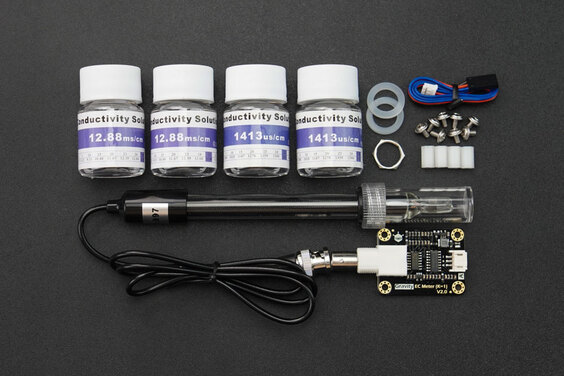
\includegraphics[scale= 0.4]{Figura_8_sensor_conductividad.jpg}
	\caption{Sensor analógico de electro conductividad \cite{DFRobot_ECsensor}.}
	\label{fig:mesh8}
\end{figure}

\subsection{Potencia de hidrógeno (pH)}
El pH o potencia de hidrógeno se conoce como la facilidad con la que una sustancia en disolución libera protones de hidrógeno o iones de oxidrilo. Según esta definición, una sustancia ácida se caracteriza por una sustancia que libera protones de hidrógeno (H+) mientras que una sustancia básica es aquella que entrega iones de oxidrilo (OH-). La escala de pH es una función logarítmica que describe la relación entre estas propiedades de una solución. Esta se encuentra en un rango de 0 a 14, en donde 0 corresponde a una sustancia ácida, mientras que 14 indica una extremadamente básica \cite{chang_quimica_1995}. La solución de agua utilizada para alimentar las plantas en un cultivo hidropónico debe contar con un pH estable, usualmente definido por el tipo de planta que se desea cultivar. En el libro \textit{Plant Factory Using Artificial Light}, el autor Wada describe cómo la regulación de pH en las soluciones nutritivas no es sólo esencial para el crecimiento de las plantas, sino también para asegurar que los nutrientes se mantengan en su estado óptimo. Wada indica que un pH por encima de 7.0 induce la presipitación del Hierro y Manganeso, lo cual afectará la producción de clorofila y volverá a las plantas más susceptibles a estrés, mientras que un pH debajo de 4.5 implicará un daño a las raíces. La regulación de los niveles de pH en sistemas hidropónicos se pueden realizar mediante mediciones de electro conductividad, para determinar los porcentajes de bicarbonato en el agua, o utilizando un sensor de pH \cite{wada_theory_2019}. Ambos métodos presentarán resultados útiles para el control de dicho parámetro, sin embargo, contar con un sensor de pH permitirá obtener una lectura directa mientras que las lecturas de conductividad únicamente indicarán el pH según las sales presentes en la solución.

\subsection{Sensor de pH \textit{SEN0161 PH Meter} de \textit{DFRobot}}
Este sensor cuenta con una construcción sencilla la cual hace de este sensor fácil de utilizar. Al ser un sensor analógico, este requiere de un proceso de calibración utilizando soluciones cuyo pH sea conocido. Cuenta con un indicador led el cual se utiliza para determinar si el sensor se encuentra encendido o no. Adicionalmente, el conector utilizado para la placa de conversión de señales permite su fácil integración con placas de desarrollo como el Arduino o ESP32 \cite{DFRobot_PHsensor}. A continuación se detallan las características del sensor:

\begin{table}[H]
	\centering
	\begin{tabular}{|c|c|}
		\hline
		\multicolumn{2}{|c|}{\textbf{Sonda del sensor de pH}}\\ \hline
		Rango de detección: & 0 a 14 pH \\ \hline
		Rango de temperatura: & 0 a 60 °C \\ \hline
		Tiempo de respuesta: & Menor o igual a 1 minuto \\ \hline
		\multicolumn{2}{|c|}{\textbf{Placa de conversión de señales del sensor}}\\ \hline 
		Voltaje de alimentación: & 5.0 VDC \\ \hline
		Cable de conexión & BNC \\ \hline
		Conector de señal: & Interfaz PH2.0 - 3 pin \\ \hline
		Certeza de medición: & $\pm 0.1$pH a 25 °C. \\ \hline
		Dimensiones: & 42 mm $\times$ 32 mm (1.65 in $\times$ 1.26 in) \\ \hline
		Potenciómetro de ajuste de ganancia & Sí \\ \hline
		Indicador de potencia: & LED \\ \hline
		Largo del cable: & 660mm \\ \hline
	\end{tabular}
	\caption{Características de funcionamiento del sensorSEN0161 de \textit{DFRobot}.}
	\label{Cuadro3}
\end{table}

\begin{figure}[H]
	\centering
	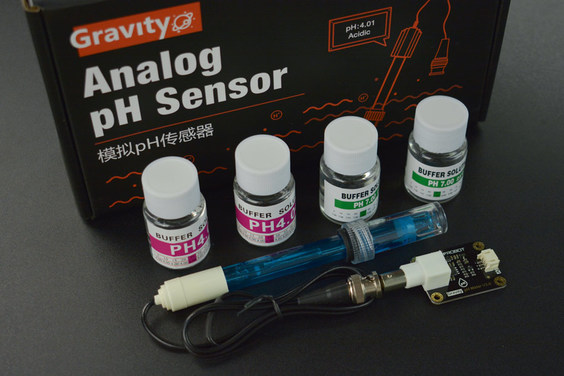
\includegraphics[scale= 1.5]{Figura_9_sensor_ph.jpg}
	\caption{Sensor analógico de potencia de hidrógeno (pH) \cite{DFRobot_PHsensor}.}
	\label{fig:mesh9}
\end{figure}

\subsection{Temperatura de agua}
La temperatura del agua es de gran importancia para las plantas puesto que está directamente relacionado a la capacidad de absorción de nutrientes. Esta temperatura es de especial importancia en las raíces, puesto que variaciones en la temperatura de estas afecta tanto la micro-biología que se desarrolle en las raíces como la habilidad de las mismas para absorber nutrientes. Adicionalmente, la temperatura afectará la precisión de lecturas de electro conductividad así como pH y oxígeno disuelto \cite{voogt_nutrient_2019}. Es por esta razón que la lectura y el control adecuado de la temperatura del agua es esencial en un sistema hidropónico. 

\subsection{Sensor de temperatura de agua DS18B20}
Uno de los sensores más fáciles de utilizar es el sensor de temperatura tipo sonda DS18B20. Este sensor utiliza el protocolo de comunicación 1-wire, lo cual reduce considerablemente la complejidad de conexión y la transmisión de datos. A continuación se detallan sus características \cite{la_electronica_DS18B20}:

\begin{table}[H]
	\centering
	\begin{tabular}{|c|c|}
		\hline
		\multicolumn{2}{|c|}{\textbf{Sonda del sensor de pH}}\\ \hline
		Rango de medición: & -55 a 125 °C \\ \hline
		Voltaje de operación: & 3.5 a 5.0 VDC \\ \hline
		Protocolo de comunicación: & 1-wire \\ \hline
		Resolución programable: & 9 a 12 bits \\ \hline
		Largo de cable: & 1 metro \\ \hline
	\end{tabular}
	\caption{Características de funcionamiento del sensor DS18B20.}
	\label{Cuadro4}
\end{table}

\begin{figure}[H]
	\centering
	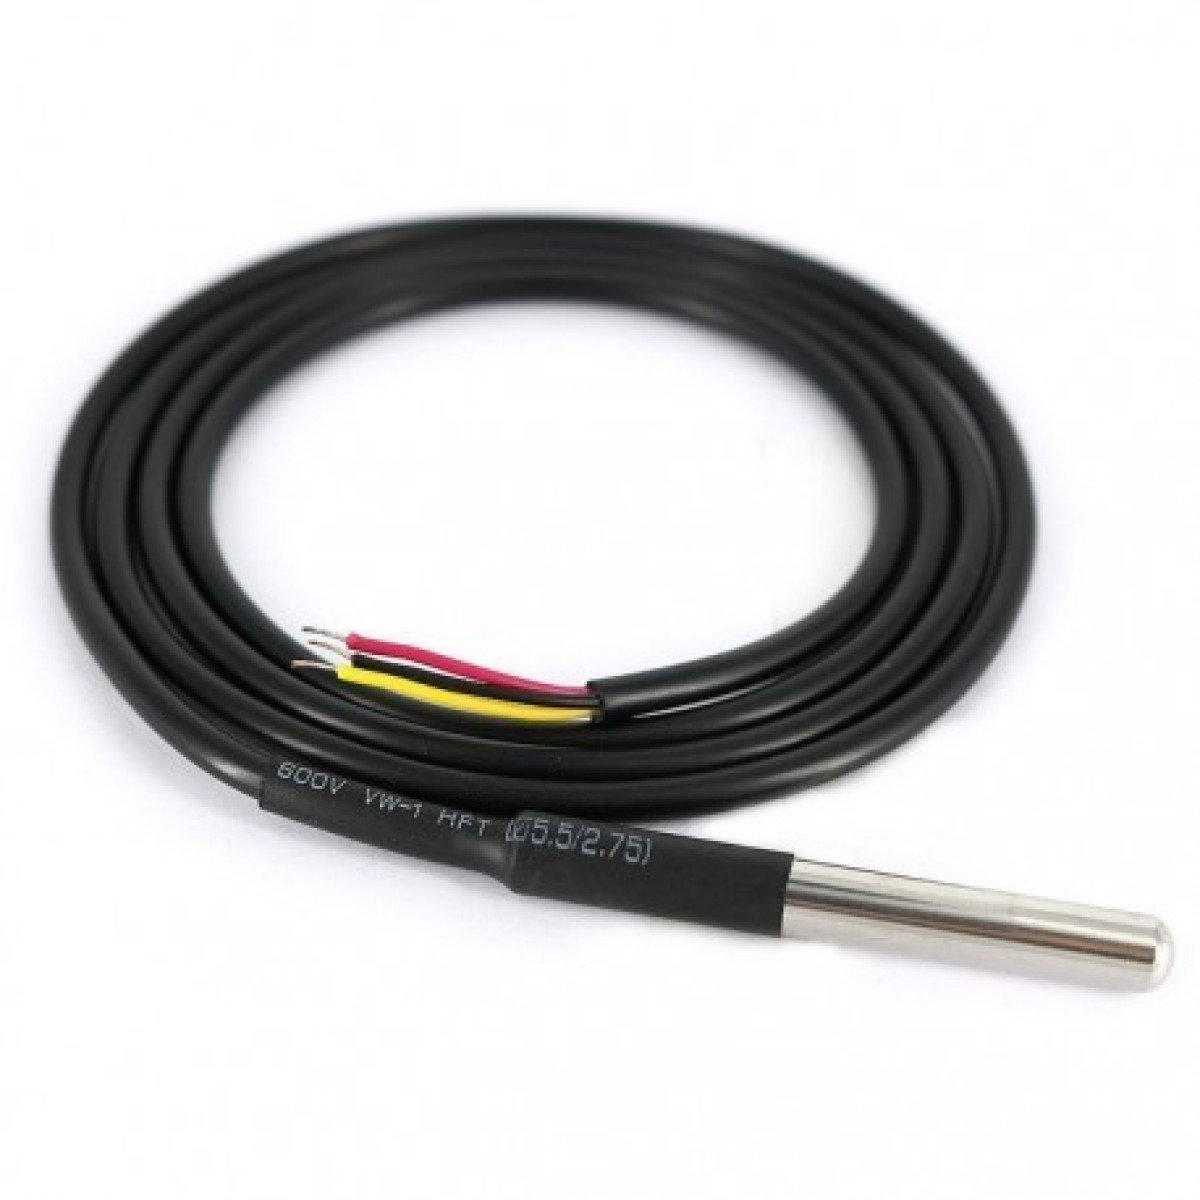
\includegraphics[scale = 0.15]{Figura_10_sensor_temperatura.jpg}
	\caption{Sensor tipo sonda de temperatura del agua \cite{la_electronica_DS18B20}.}
	\label{fig:mesh10}
\end{figure}

\subsection{Temperatura y humedad ambiental}
Las plantas son organismos particularmente susceptibles a las condiciones ambientales, tanto a los niveles de luz como a la temperatura y humedad disponible. Estos parámetros afectan diferentes procesos de las plantas, desde la absorción de nutrientes hasta el desarrollo de las hojas. Según el estudio realizado por Chia y Lim, la humedad ambiental presentó un impacto significativo en el desarrollo de cultivos, donde se observó un aumento en la masa de las plantas luego de su cosecha \cite{chia_critical_2022}. Los autores describen como las plantas en un rango de humedad relativa (RH) alrededor del 85\% presentan un aumento en su masa seca. Destacaron que a mayores porcentajes de humedad, las plantas presentan dificultades con las razones de transpiración, regulación de agua, desarrollo de área superficial de las hojas y una disminución en absorción de nutrientes. Por otro lado, destacaron que a menores concentraciones de humedad, las plantas aumentan su consumo de agua junto con sus tazas de transpiración, lo cual puede presentar un riesgo en plantas que presentan dificultades en el control de las aperturas estomáticas, lo cual afecta los procesos de fotosíntesis \cite{chia_critical_2022}.

Al igual que la humedad ambiental, la temperatura del aire alrededor de las plantas afectará su crecimiento. En el estudio realizado por Rusu y colaboradores, se analizó el crecimiento de plantas de albahaca bajo condiciones controladas con tal de determinar el impacto de dichos parámetros en el desarrollo de las plantas. Se estableció que si bien el control de la temperatura de la solución es esencial para el correcto desarrollo delas plantas, la temperatura del ambiente es igual de importante. Esto se debe a que la temperatura ambiental afectará los procesos de transpiración de las plantas, el proceso de fotosíntesis, la conductividad estomática y el crecimiento de las estructuras de la planta \cite{rusu_overview_2021}. Por otro lado, ciertos compuestos bioactivos aumentan en concentración al estar en rangos de temperatura elevados (mayores a 30° C). Finalmente, los extremos de temperatura presentan un aumento en el estrés de las plantas, llevando a una mayor demanda de agua, lo cual puede aumentar la concentración de sales creando bloqueos \cite{bita_plant_2013}. 

\subsection{Sensor de temperatura y humedad DHT11}
El sensor DHT11 es uno de los sensores más básicos y de bajo costo disponibles en el mercado para la medición de temperatura y humedad relativa en el entorno. Cuenta con un sensor capacitivo el cual es capaz de detectar el porcentaje de humedad relativo en el aire, así como una termo-resistencia la cual es capaz de detectar cambios en la temperatura ambiental. \cite{adafruit_dht11} Este sensor utiliza el protocolo \textit{one-wire} lo cual minimiza los puertos a utilizar, y elimina la necesidad de puertos analógicos para realizar lecturas. Ahora bien, cuenta con un período de muestreo máximo de una lectura por segundo, lo cual hace que sea poco preciso en ambientes con alta variabilidad. A continuación se detallan las características del sensor.

\begin{table}[H]
	\centering
	\begin{tabular}{|c|c|}
		\hline
		\multicolumn{2}{|c|}{\textbf{Sensor DHT11}}\\ \hline
		Rango de medición de temperatura: & 0 a 50 °C \\ \hline
		Precisión de temperatura: & $\pm$ 2° C \\ \hline
		Rango de medición de humedad: & 20 a 80\% \\ \hline
		Precisión de humedad: & 5\% \\ \hline
		Voltaje de operación: & 3.0 a 5.0 VDC \\ \hline
		Corriente máxima: & 2.5mA \\ \hline
		Frecuencia de muestreo: & 1Hz \\ \hline
		Protocolo de comunicación: & \textit{1-wire} \\ \hline
	\end{tabular}
	\caption{Características de funcionamiento del sensor DHT11 \cite{adafruit_dht11}.}
	\label{Cuadro5}
\end{table}

\begin{figure}[H]
	\centering
	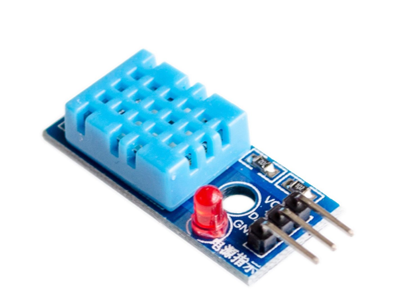
\includegraphics[scale = 0.5]{Sensor_temp_hum_dht11.png}
	\caption{Sensor de temperatura y humedad DHT11 \cite{tettsa_dht11}.}
	\label{fig:mesh11}
\end{figure}
\newpage
\subsection*{Módulo RTC (reloj de tiempo real)}
Los módulos RTC cuentan con un reloj interno el cual puede ser utilizado para determinar la hora y fecha con gran precisión. El módulo DS3231 cuenta con un protocolo de comunicación el cual permite conectar varios sensores en serie, reduciendo la cantidad de entradas y salidas requeridas en placas de desarrollo. A continuación se detallan las características del módulo \cite{la_electronica_DS3231}:

\begin{table}[H]
	\centering
	\begin{tabular}{|c|c|}
		\hline
		\multicolumn{2}{|c|}{\textbf{Placa del módulo RTC DS3231}}\\ \hline
		Voltaje de alimentación: & 3.3 a 5.5 VDC \\ \hline
		Precisión de reloj: & Error de 1 minuto a temperatura entre 0 y 40 °C \\ \hline
		Salida programable de onda cuadrada: & Sí \\ \hline
		Chip de memoria: & AT24C32 con capacidad de almacenamiento de 32kB \\ \hline
		Dimensiones: & 38 mm $\times$ 22 mm $\times$ 14 mm \\ \hline
		Peso: & 8g \\ \hline
	\end{tabular}
	\caption{Características de funcionamiento del módulo RTC DS3231.}
	\label{Cuadro:caracter_rtc}
\end{table}

\begin{figure}[H]
	\centering
	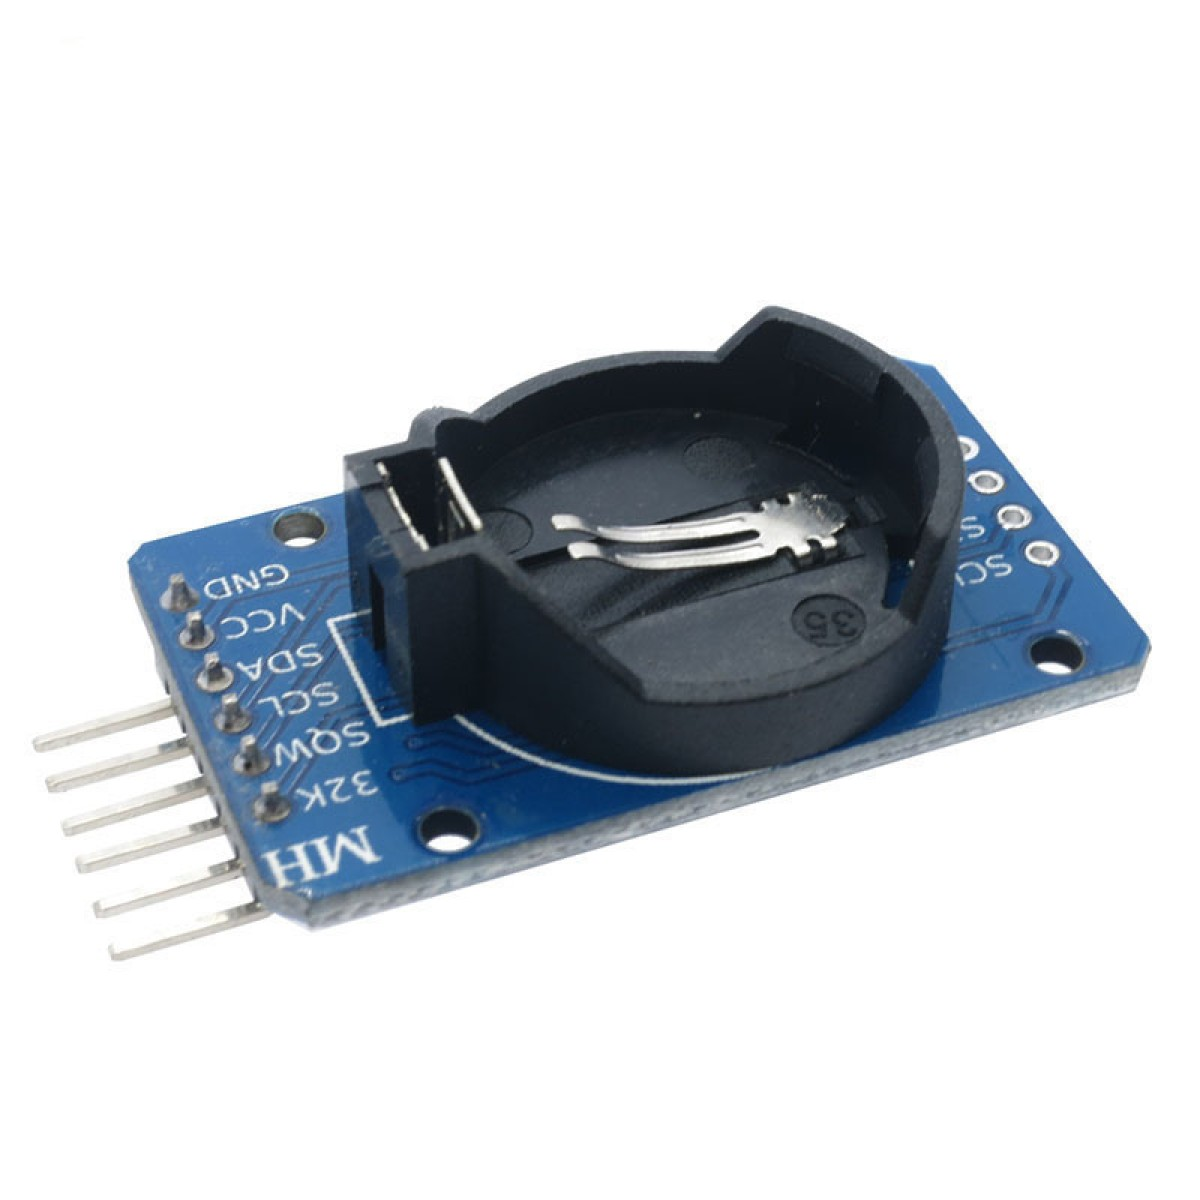
\includegraphics[scale = 0.15]{Figura_11_rtc.jpg}
	\caption{Módulo RTC DS3231 \cite{la_electronica_DS3231}.}
	\label{fig:modulo_rtc}
\end{figure}

\section{Placa de desarrollo \textit{ESP-WROOM-32}}
La ejecución de los procesos de control así como la recolección de datos de los sensores instalados requiere del uso de un microcontrolador. Las placas de desarrollo de la familia ESP32 son de gran utilidad, puesto que permiten la fácil integración del módulo ESP32 en cualquier proyecto. El módulo ESP32 es uno de los microcontroladores más versátiles y de menor costo disponibles en el mercado. Este cuenta con conectividad WiFi, \textit{Bluetooth} v4.2, \textit{Bluetooth Low Energy}, pines analógicos, diferentes protocolos de comunicación serial y paralela, dos núcleos de procesamiento y compatibilidad con el lenguaje de programación de Arduino. Adicionalmente, las placas de desarrollo diseñadas alrededor de este microcontrolador cuentan con un costo reducido y bajo consumo eléctrico, lo cual lo hace ideal para aplicaciones con limitantes de costos. A continuación se detallan las características generales de la placa de desarrollo \textit{ESP-WROOM-32} \cite{electronic_wings_espwroom32}:

\begin{table}[H]
	\centering
	\begin{tabular}{|c|c|}
		\hline
		\multicolumn{2}{|c|}{\textbf{Placa de desarrollo \textit{ESP-WROOM-32}}}\\ \hline
		Procesador: & 2 núcleos hasta 240 MHz \\ \hline
		WiFi: & 2.4 GHz hasta 150 Mbits/s \\ \hline
		\textit{Bluetooth}: & \textit{Bluetooth Low Energy} y \textit{Bluetooth} v4.2 \\ \hline
		Arquitectura del procesador: & 32 bits \\ \hline
		Memoria RAM: & 520 KB \\ \hline
		Cantidad de pines IO: & 38 \\ \hline
		Cantidad de pines tipo ADC: & 16 \\ \hline
		Botones disponibles: & Botón de arranque y reinicio \\ \hline
		Leds disponibles: & Indicador LED de estado \\ \hline
		Puente USB a UART: & CP2102 \\ \hline
	\end{tabular}
	\caption{Características de funcionamiento y conexión de la placa de desarrollo \textit{ESP-WROOM-32}.}
	\label{Cuadro6}
\end{table}

\begin{table}[H]
	\centering
	\begin{tabular}{|c|c|}
		\hline
		\multicolumn{2}{|c|}{\textbf{Periféricos adicionales}}\\ \hline
		\multicolumn{2}{|c|}{Sensor capacitivo integrado}\\ \hline
		\multicolumn{2}{|c|}{Conversor Digital Analógico}\\ \hline
		\multicolumn{2}{|c|}{I2C (\textit{Inter-Internal Circuit})}\\ \hline
		\multicolumn{2}{|c|}{UART (\textit{Universal asyncrhonous receiver/transmitter})}\\ \hline
		\multicolumn{2}{|c|}{SPI (\textit{Serial Peripheral Interface})}\\ \hline
		\multicolumn{2}{|c|}{PWM (\textit{Pulse Width Modulated})}\\ \hline
	\end{tabular}
	\caption{Protocolos de comunicación y otros periféricos disponibles en el \textit{ESP-WROOM-32}.}
	\label{Cuadro7}
\end{table}

\begin{figure}[H]
	\centering
	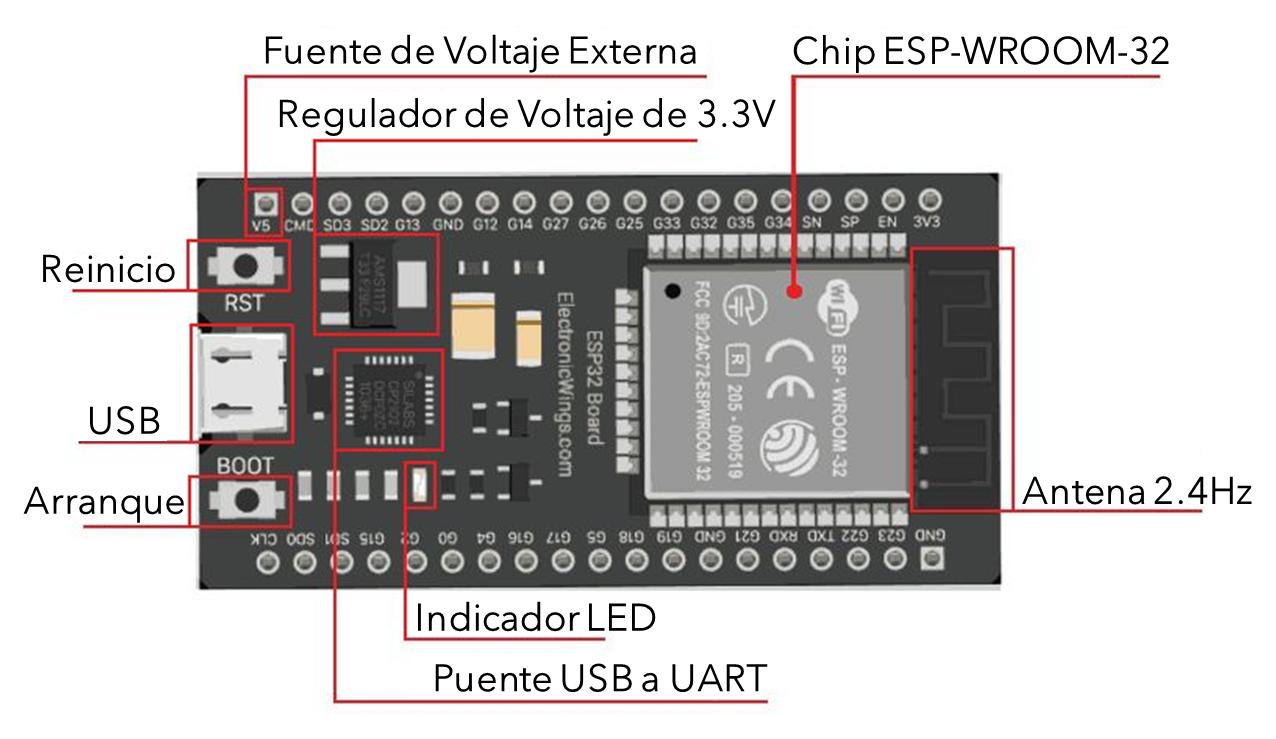
\includegraphics[scale = 0.5]{Figura_12_espwroom32.png}
	\caption{Componentes de la placa de desarrollo ESP-WROOM-32 \cite{electronic_wings_espwroom32}.}
	\label{fig:mesh12}
\end{figure}

\section{Sistemas de control y conectividad con la nube}

\subsection{El internet de las cosas (IoT)}
El internet de las cosas se refiere a la capacidad de conectar objetos de uso cotidiano al internet para compartir parámetros de funcionamiento y otros datos entre diferentes dispositivos. La capacidad de compartir datos de manera inalámbrica con poca intervención humana hace de este proceso ideal para la automatización de procesos en diferentes sectores, desde el hogar hasta la ciudad entera. En general, los dispositivos IoT se pueden categorizar en sensores y actuadores o controladores, donde estos cumplen la función de recolectar datos y activar procesos respectivamente. Un sistema IoT básico funciona mediante un ciclo de retroalimentación constante de recolección, envío y análisis de datos para controlar diferentes eventos o indicar el estado de estos. El internet de las cosas se puede encontrar en una gran variedad de aplicaciones, desde la industria de manufactura, procesos de logística y transportación de productos hasta la agricultura. \cite{redhat_IoT_2019}

\begin{figure}[H]
	\centering
	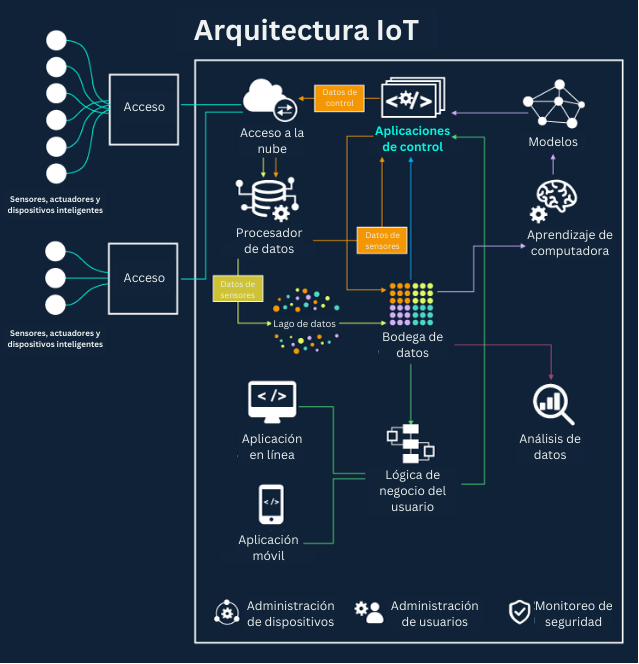
\includegraphics[scale = 0.55]{Figura_13_arquitectura_iot.png}
	\caption{Diagrama de la arquitectura IoT generalizada \cite{grizhnevich_iot_2018}.}
	\label{fig:mesh13}
\end{figure}

\subsection{Protocolo de comunicación HTTP}
El internet funciona gracias a una serie de protocolos de comunicación que permiten la transferencia de datos como imágenes, texto, videos y audios entre servidores y usuarios. Uno de los protocolos fundamentales para la transmisión de estos datos es el protocolo HTTP (\textit{Hypertext Transfer Protocol}) o Protocolo de Transferencia de Hipertexto. La primera versión de HTTP para la transferencia de datos fue utilizada en 1990 como una herramienta para enviar datos a un usuario. Esta primera versión se conoce como HTTP/0.9. Esta iteración del protocolo se conoció como el protocolo de una línea, puesto que contaba con una gran cantidad de limitaciones, permitiendo únicamente realizar búsquedas de elementos como páginas escritas en HTML, imágenes o archivos específicos \cite{Evolution_http_Mozilla_2024}. Unos años después, gracias a un esfuerzo conjunto entre el MIT, \textit{Microsoft} y otras empresas, se desarrolló el protocolo HTTP/1.1. Una de las ventajas principales de este nuevo protocolo consistía en la adición de sistemas para el envío de datos a un servidor. Adicionalmente, se definieron nuevas reglas que permitieron que este sistema fuese más estable e incluso permitiera la transferencia de datos de manera simultánea \cite{fielding_hypertext_1999}. Este protocolo estableció los fundamentos para el desarrollo de futuras versiones, actualmente, las más utilizadas son  es la versión HTTP/2.0 y HTTP/3.0.

El protocolo HTTP consiste en el uso de una solicitud con una instrucción específica la cual es transmitida desde un usuario o cliente (\textit{client}). Esta solicitud se realiza mediante una conexión TCP o UDP dependiendo de la versión del protocolo, y cuenta con una estructura estandarizada para extraer, agregar, cambiar o eliminar información en el servidor. Una solicitud para retirar datos presenta la estructura observada en la Figura \ref{fig:mesh14}. Las palabras \textit{GET}, \textit{POST}, \textit{PUT}, \textit{PATCH} y \textit{DELETE} son utilizadas para indicarle al servidor durante la solicitud realizada las acciones a realizar. Adicionalmente, se especifica la dirección del servidor junto con información importante para la transacción y el contenido del mensaje en caso de que este sea requerido \cite{overview_http_mozilla_2024}.

\begin{figure}[H]
	\centering
	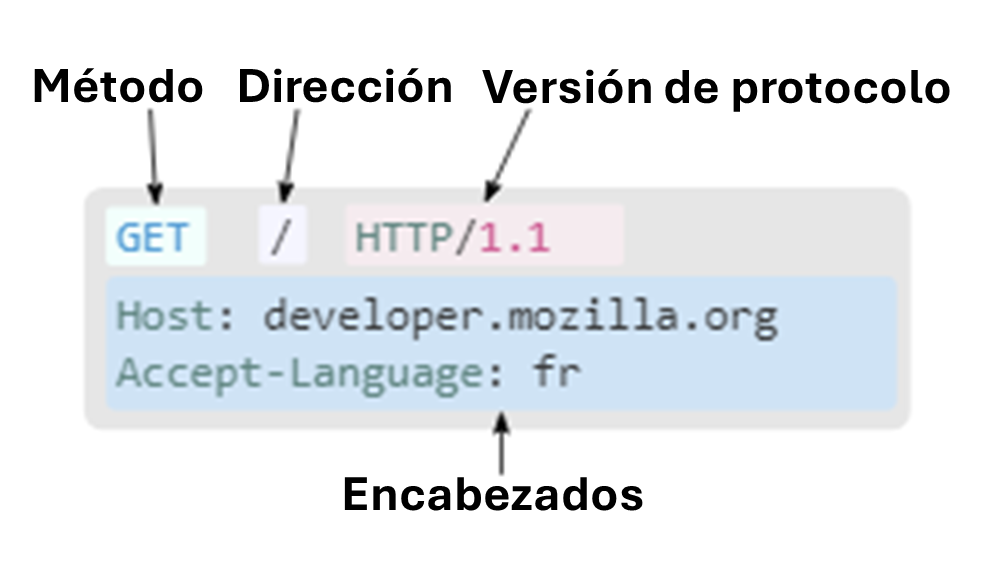
\includegraphics[scale = 0.35]{Figura_14_solicitud_http.png}
	\caption{Estructura de una solicitud para retirar datos en el protocolo HTTP/1.1 \cite{overview_http_mozilla_2024}.}
	\label{fig:mesh14}
\end{figure}

Las solicitudes realizadas por el cliente son dirigidas directamente al servidor indicado en la dirección, sin embargo, usualmente se utilizan dispositivos intermedio para realizar dicha conexión. Una vez que el servidor recibe la solicitud, este devuelve una respuesta con un encabezado en el cual se detallan las características del archivo, así como ciertos códigos para indicar el estado de la conexión. Adicionalmente, la respuesta del servidor contará con la información solicitada por el cliente, ya sea esta un segmento de texto, un archivo, una página web o un video. Gracias a su simplicidad, este protocolo es el más utilizado hoy en día para intercambios de información en la red \cite{overview_http_mozilla_2024}.

\begin{figure}[H]
	\centering
	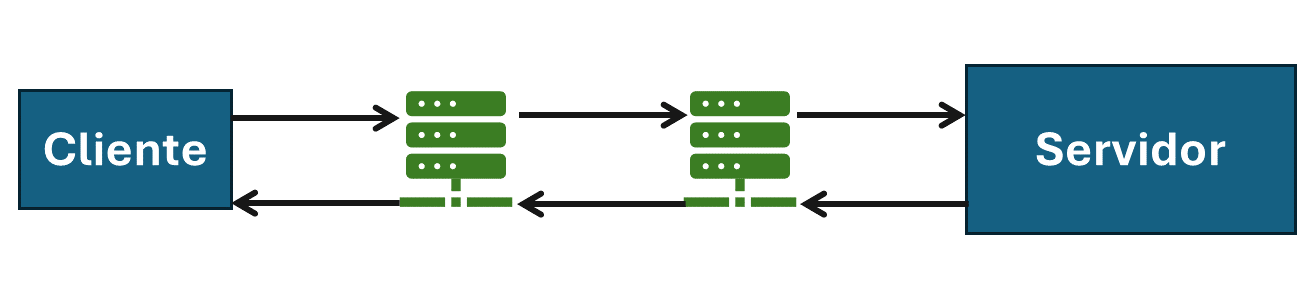
\includegraphics[scale = 0.4]{Figura_14.1_comunicacion_http.png}
	\caption{Diagrama de la comunicación entre cliente y servidor mediante el protocolo HTTP \cite{overview_http_mozilla_2024}.}
	\label{fig:mesh14_1}
\end{figure}

\subsection{Comunicación WiFi con \textit{Dweet.io}}
\textit{Dweet.io} es un servicio abierto al público y totalmente gratuito que permite la transferencia de datos entre dispositivos funcionando como servidor para comunicaciones mediante HTTP. \textit{Dweet.io} utiliza un tema, llamado \textit{Thing}, el cual funciona como un servidor que recibe solicitudes mediante HTTP. Esta funcionalidad permite que diferentes dispositivos con conexión a la red puedan solicitar información almacenada o cargar nuevos datos a este servidor utilizando la dirección del tema. Una de sus mayores ventajas es que almacena datos en la forma de texto, el cual es distribuido en el cuerpo de las solicitudes HTTP. Esto permite almacenar diferentes valores de manera legible para cualquier humano, facilitando así el proceso de recolección e intercambio de datos. Es importante destacar que al ser gratuito, este servicio es completamente público y los mensajes pueden ser leídos por cualquiera con acceso a este servicio \cite{dweet_dweetio_faq}. Adicionalmente, los mensajes enviados a los servidores de \textit{Dweet.io} son almacenados únicamente durante 24 horas, a menos de que se pague una suscripción a un servidor privado.

\begin{figure}[H]
	\centering
	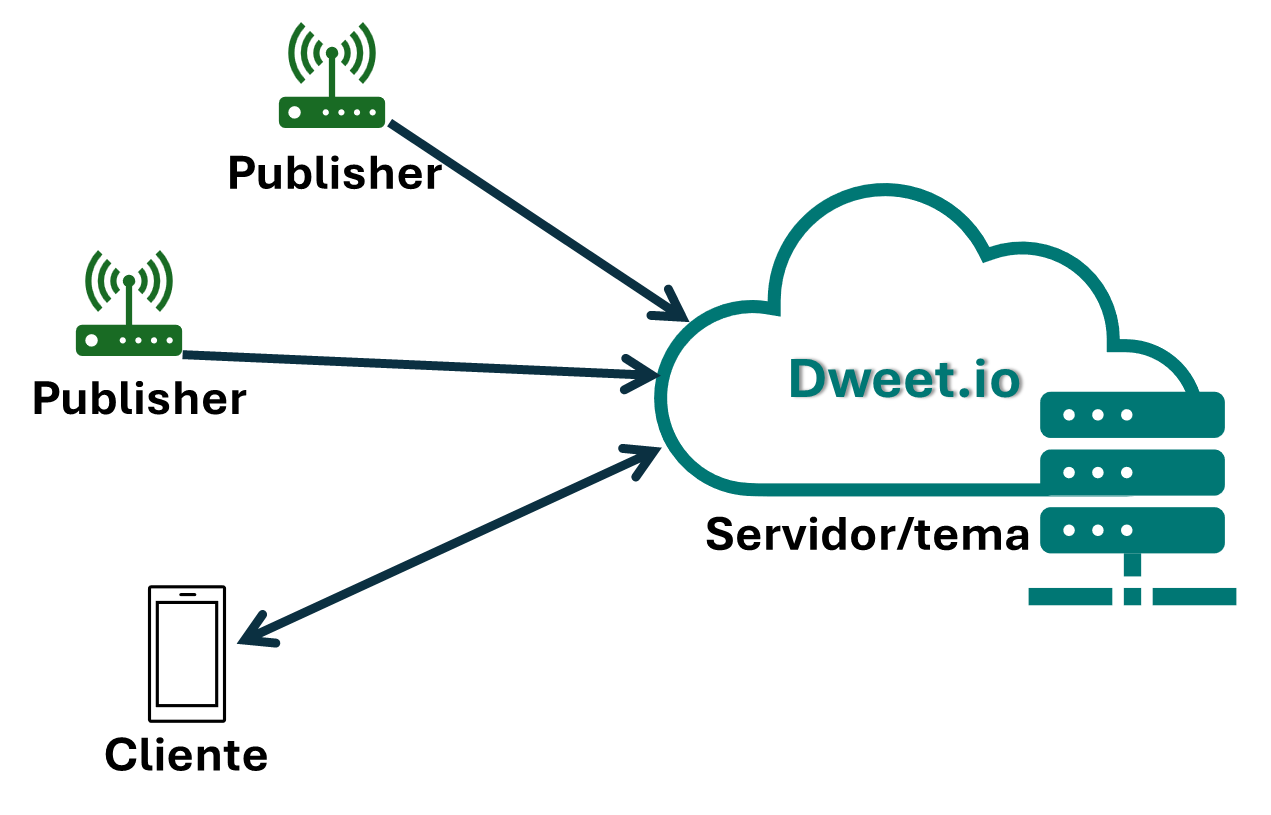
\includegraphics[scale = 0.4]{Figura_16_comunicacion_dweetIO.png}
	\caption{Diagrama de la comunicación entre cliente y servidor de \textit{Dweet.io}.}
	\label{fig:mesh16}
\end{figure}

\subsection{Controladores de Fuzzy Logic}
En el área de control de sistemas, existen casos en donde el sistema a controlar presenta una gran cantidad de entradas y salidas así como una alta complejidad matemática en las variables de estado que lo definen, en la forma de no linealidades. En estos casos, el desarrollo de un modelo matemático que sea capaz de describir adecuadamente todas las relaciones entre variables llega a ser demasiado complejo, por lo cual se buscan alternativas para el control. Uno de los métodos diseñados para el control de estos sistemas se basa en la teoría de \textit{Fuzzy Sets} el cual busca establecer rangos de funcionamiento lineales para las variables de control del sistema así como relaciones lineales entre los diferentes parámetros que estas controlan. Estos se logra mediante procesos matemáticos para obtener rangos que permitan un control adecuado del sistema, sin la realización de un modelo matemático que describa todas las dinámicas del sistema \cite{verbruggen_fuzzy_1999}.



